\documentclass[xcolor=svgnames,dvipsnames,table, hyperref=pdftex, mathserif, presentation]{beamer}
\usepackage{amsmath,amssymb,amsfonts,amsthm}
\usepackage{ctex}
\usepackage{graphics}
\usepackage{graphicx}
\usepackage{xcolor}
\usepackage{wasysym}
\usepackage{bbm}
\usepackage{url}
\usepackage{beamerleanprogress}
\usepackage{tikz-dependency}
\usepackage{tikz-qtree}
\usepackage{hhline}
\usepackage{fancyvrb}
\usepackage{mathrsfs}
\usepackage{multirow}
\usepackage{alltt}
\usepackage[subrefformat=parens]{subcaption}
% for uml charts
\usepackage{tikz}
\usetikzlibrary{calc,arrows.meta, graphs, trees, shapes, positioning, automata,
shapes.geometric, shapes.multipart, er, patterns, decorations.markings, intersections, decorations.text}
\usepackage{tikz-uml}

\usetheme{CambridgeUS}
%\usetheme{Pittsburgh}
\usecolortheme{orchid} % seahorse  orchid rose
\setbeamertemplate{blocks}[rounded][shadow=true]
\AtBeginSection[]{%
  \begin{frame}<beamer>
    \frametitle{Outline}
      \tableofcontents[current] 
    \end{frame}
  \addtocounter{framenumber}{-1}% If you don't want them to affect the slide number
}
\AtBeginSubsection[]
{
  \begin{frame}
  \frametitle{Outline}
    \tableofcontents[currentsection,currentsubsection]
  %\tableofcontents[sectionstyle=show/hide,subsectionstyle=hide/show/hide]
  \end{frame}
  \addtocounter{framenumber}{-1}% If you don't want them to affect the slide number
}
\newcommand{\setof}[1]{\ensuremath{\left \{ #1 \right \}}}
\newcommand{\tuple}[1]{\ensuremath{\left \langle #1 \right \rangle }}
\newcommand{\red}[1]{\textcolor{red}{#1}}
\newcommand{\brown}[1]{\textcolor{brown}{#1}}
\newcommand{\green}[1]{\textcolor{green}{#1}}
\newcommand{\blue}[1]{\textcolor{blue}{#1}}
\newcommand{\cyan}[1]{\textcolor{cyan}{#1}}

%gets rid of navigation symbols
%\setbeamertemplate{navigation symbols}{}

\begin{document}

\title[PredUni]{Detecting Synonymous Predicates from Online Encyclopedia with Rich Features \[AIRS 2016\]}

\institute[icst@pku]{
  Institute of Computer Science \& Technology \\
  Peking University
}
\author[Zhe]{
  Zhe, Han
}

\frame[t,plain]{ \titlepage } % [t,plain]

\frame{
  \frametitle{ Outline }
   \begin{itemize}
      \item Predicate Unification Background
      \item Motivation \& Related Work
      \item Problem Definition
      \item Features
	  \begin{itemize}
	   \item Predicate Representation
	  \end{itemize}
      \item Experiment \& Analysis
      \item Conclusion \& Future Work
   \end{itemize}
}

\frame{
  \frametitle{background}
  \begin{columns}[c]
   \column{0.4\hsize}

  \begin{itemize}
   \item Online Encyclopedia => \textbf{\red{K}nowledge \red{B}ases}
      \begin{itemize}
       \item infobox/text => triple
      \end{itemize}
  \end{itemize}
  \begin{columns}[c]
   \column{0.3\hsize}
   \centering 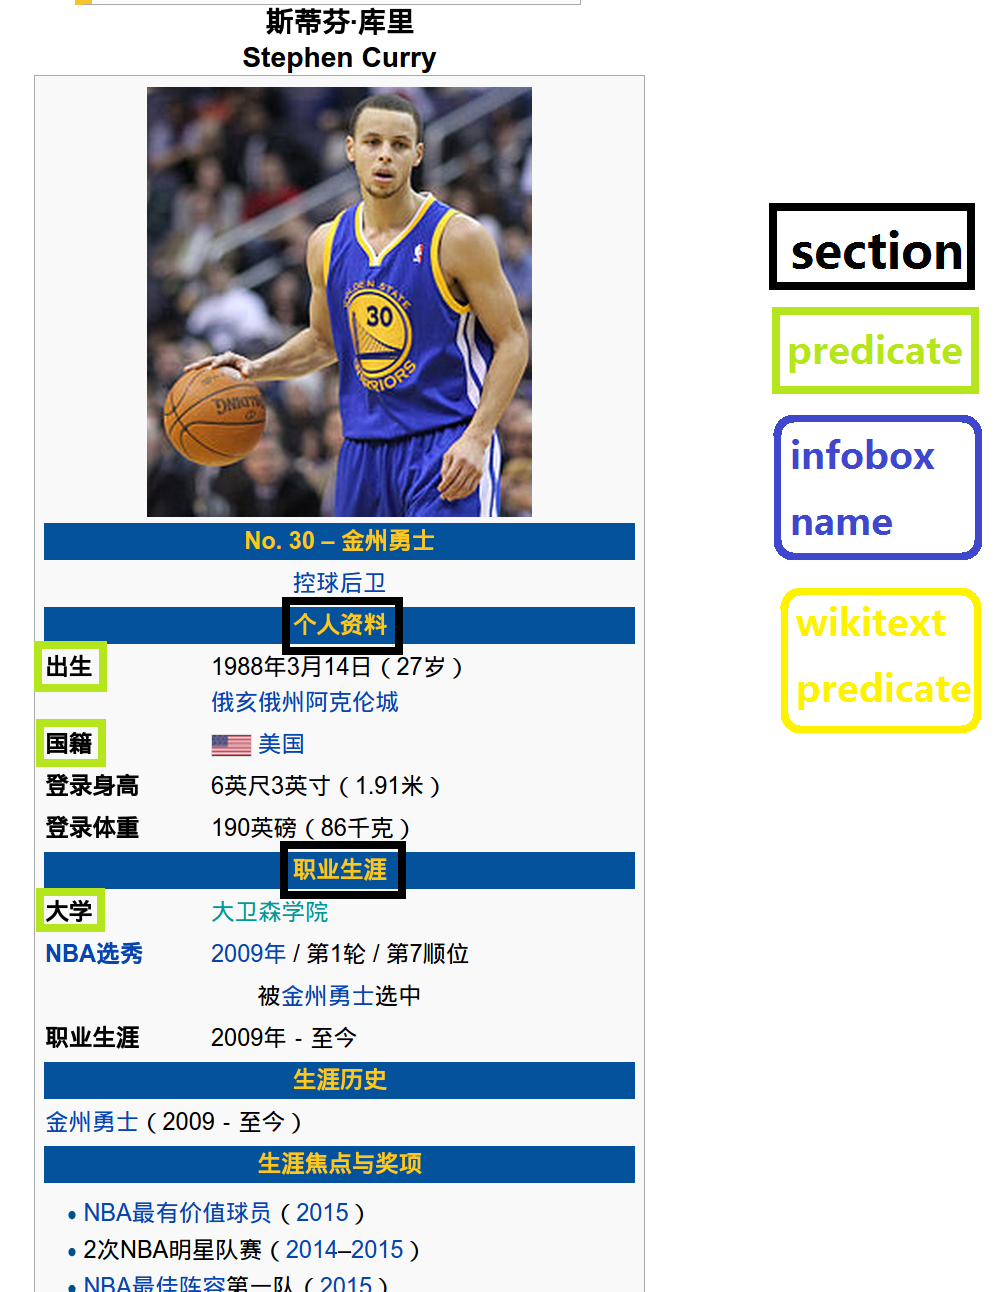
\includegraphics[width=0.95\hsize]{pic/curry_big2.png}
   \column{0.5\hsize}
   \centering 
\includegraphics[width=0.7\hsize]{pic/wikipedia.png}
  \end{columns}
  \vspace{0.3em}
  \begin{columns}[c]
   \column{0.99\hsize}
   \centering 
\includegraphics[width=0.4\hsize]{pic/yago.png}
   \centering 
\includegraphics[width=0.4\hsize]{pic/dbpedia.png}
  \end{columns}
  \vspace{0.3em}
   \centering 
\includegraphics[width=0.6\hsize]{pic/freebase.png}
  
   \column{0.55\hsize}
  
  \begin{block}{problems on building structured KBs}
   \begin{itemize}\small
   \item taxonomy construction
      \begin{itemize}\footnotesize
       \item basketball player->sportsman->person
      \end{itemize}
   \item \textbf{predicate standardize/unification}
     \begin{itemize}\footnotesize
      \item birthday, birthdate; birth place, born place
     \end{itemize}

   \item value/object standardize/purge
      \begin{itemize}\footnotesize
       \item \red{1900-10-02}, \blue{02-10-1900}
      \end{itemize}
   \item entity linking
      \begin{itemize}\footnotesize
       \item Michael Jordan -> \{Michael Jordan(\red{player}), Michael Jordan(\blue{scientist})\}
      \end{itemize}
  \end{itemize}
  \end{block}

  \end{columns}
   
}

\frame{
  \frametitle{background}
  
  \begin{block}{}
   \centering Predicate unification is of great  importance and difficulty!
  \end{block}
  
  \begin{itemize}
   \item editor preference
      \begin{itemize}
       \item too many surface forms
       \item concrete vs general
      \end{itemize}
   \item lack of Chinese KB
      \begin{itemize}
       \item DBpedia has no linked triples / no predicate set
       \item Freebase has fewer Chinese triples
      \end{itemize}
   \item Chinese
      \begin{itemize}
       \item lack of resources, like WordNet
       \item Pronunciation/typos (\red{坐标},\blue{座标})
      \end{itemize}
  \end{itemize}
}

\frame{
  \begin{columns}[c]
   \column{.15\hsize}
   \column{.7\hsize}
   \begin{block}{}
    \centering \Large Related work
   \end{block}
   \column{.15\hsize}
  \end{columns}
}

\frame{
  \frametitle{related work}
  \begin{enumerate}
   \item DBpedia
      \begin{itemize}
       \item \blue{Handwritten} rules to map wikitext to property set ($\approx1000$)
       \item each kind of infobox/template has their mapping rules
	  \begin{itemize}\small
	   \item no mapping rules are included in Chinese DBpedia
	   \item \red{birthdate} would be written many times if exists in different templates
	  \end{itemize}
      \end{itemize}
   \item YAGO
      \begin{itemize}
       \item \blue{Lmited} predicate set ($\approx120$) to avoid inside predicate unification
      \end{itemize}
   \item Freebase
      \begin{itemize}
       \item (Tan 2014) detect synonyms based on user domain expertise and \blue{co-occurrence} of objects and subjects
       \item object type info is needed
      \end{itemize}
  \end{enumerate}
}

\frame{
  \frametitle{related work}
  \begin{enumerate}
  \setcounter{enumi}{3}
   \item Abedjan treats syn-pred detection as a \blue{association rule mining} problem
   \item Baroni and Wei find co-occurrence of \blue{synonym candidates} in web documents
  \end{enumerate}
  \begin{enumerate}
  \setcounter{enumi}{5}
   \item Naumann proves effectiveness of \blue{aggregate features}
   \item Li's experiment shows \textbf{weak} performance using \red{dictionaries only}
  \end{enumerate}
}

\frame{
  \begin{columns}[c]
   \column{.15\hsize}
   \column{.7\hsize}
   \begin{block}{}
    \centering \Large Problem Definition
   \end{block}
   \column{.15\hsize}
  \end{columns}
}

\frame{
  \frametitle{Wikipedia Resources}
  \begin{center}
    \begin{columns}[c]
      \column{.45\hsize}
      \begin{figure}
	  \centering 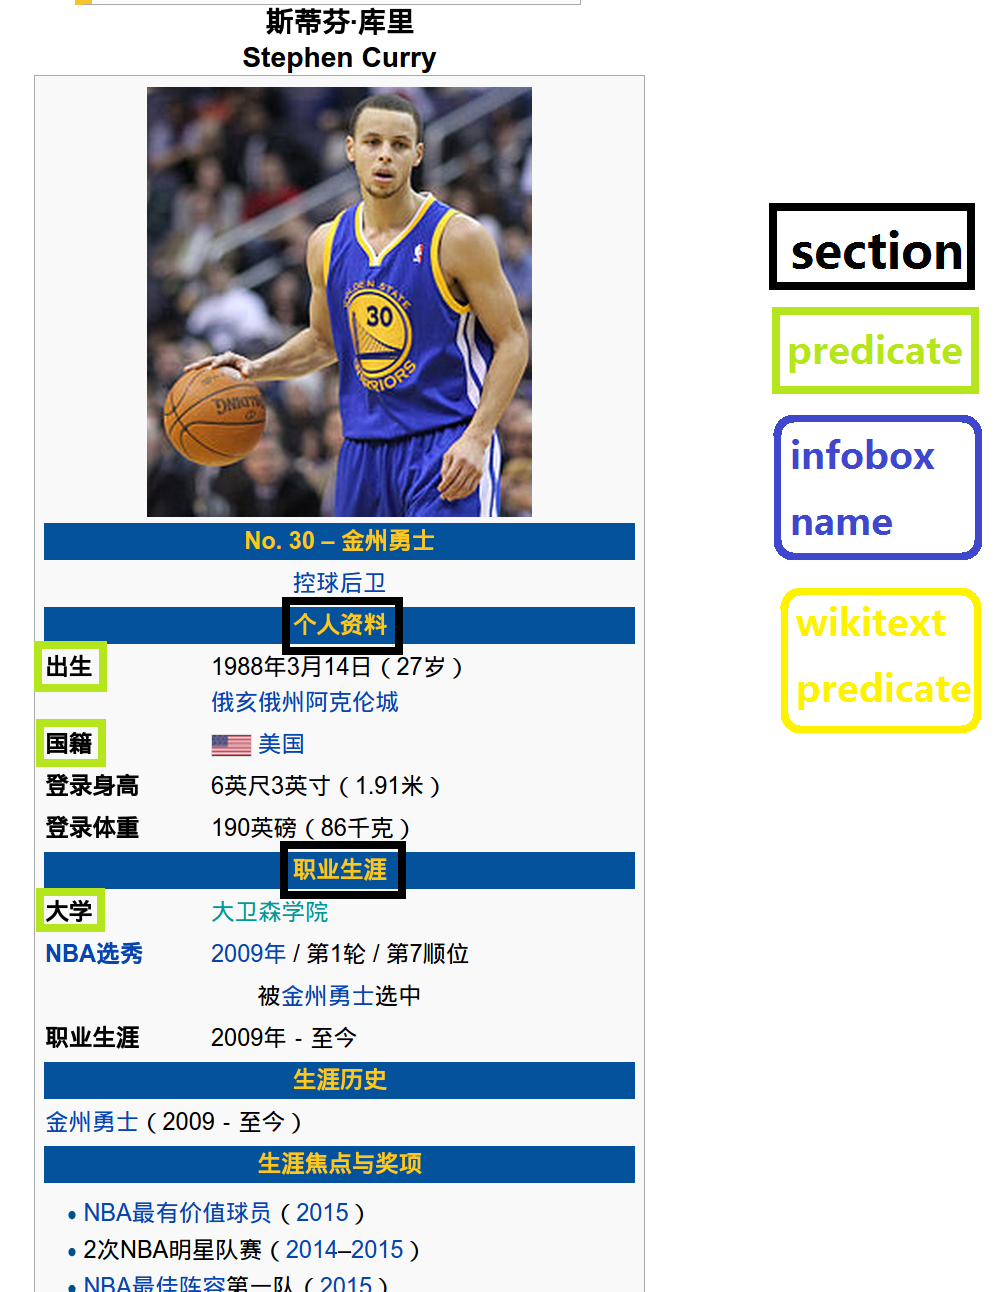
\includegraphics[width=0.95\hsize]{pic/curry_big2.png}
	  \caption{Wikipedia web info}
      \end{figure}

      \column{.7\hsize}
      \begin{figure}
	  \centering 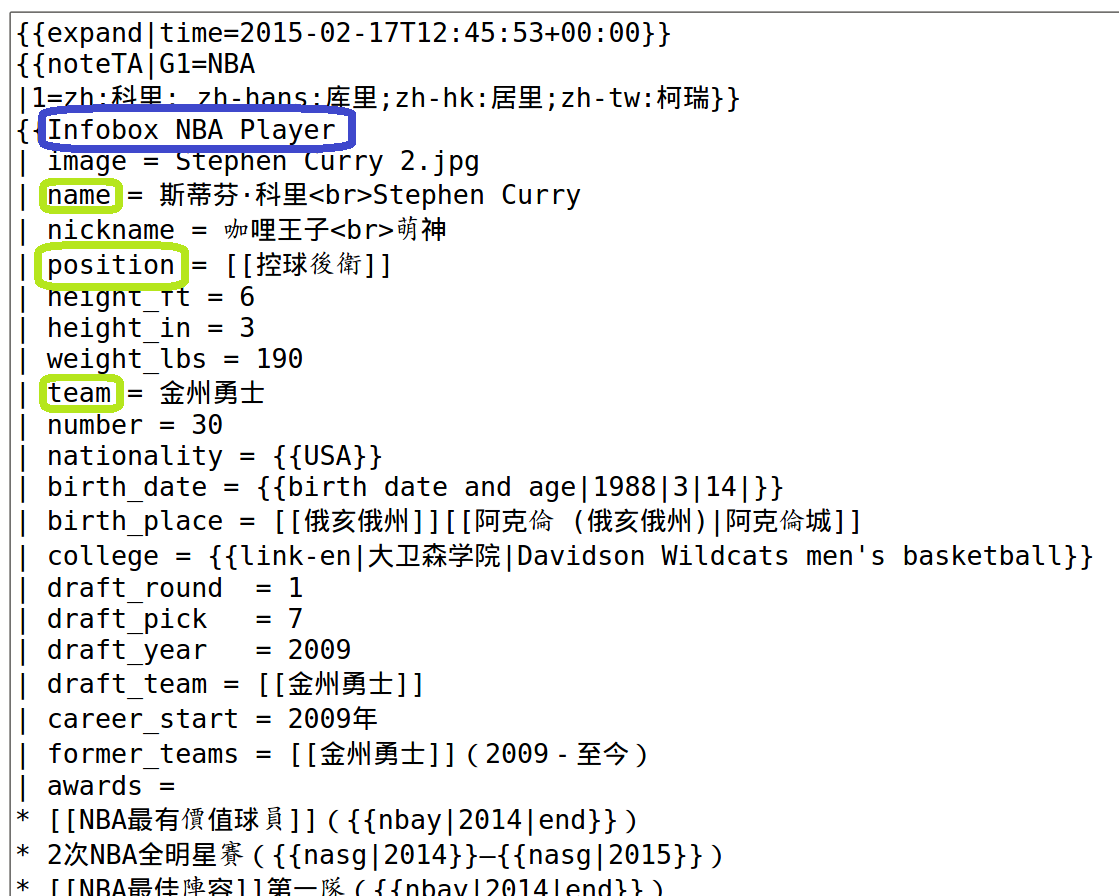
\includegraphics[width=0.9\hsize]{pic/curry_wikitext_big2.png}
	  \caption{wikitext info}
      \end{figure}
    \end{columns}
  \end{center}
}

\frame{
      \begin{block}{Problem Definition}
	\begin{itemize}
	 \item binary classification problem
	 \item given a pair of predicates $pred 1$ , $pred 2$ from Wikipedia web infoboxes, predicting whether these two are synonyms
	\end{itemize}
      \end{block}
      
      \begin{itemize}
       \item process 
	  \begin{enumerate}
	   \item  give the \textbf{representation vector} of each predicate
	   \item calculate the \textbf{feature vector} from the vector pair
	   \item give the association score of this pair from pre-trained classifier
	  \end{enumerate}
       \item different from other's work.
	  \begin{itemize}
	   \item no structured Chinese KB based on Wikipedia(non-structured objects)
	   \item other works are on DBpedia/Freebase with \textbf{structured objects (type info)}
	   \item directly on \red{web predicate}
	  \end{itemize}
      \end{itemize}
}

\frame{
  \begin{columns}[c]
   \column{.15\hsize}
   \column{.7\hsize}
   \begin{block}{}
    \centering \Large Features \\ 
    \small --- Predicate Representation
   \end{block}
   \column{.15\hsize}
  \end{columns}
}

\frame{
  \begin{itemize}
   \item 7 kinds of features
      \begin{itemize}
       \item surface form features
       \item pinyin features
       \item bilingual dictionary features
       \item wikitext features
       \item wikiSection featureses
       \item wikiInfobox features
       \item Freebase category features
      \end{itemize}
   \item combine to a large feature vector
  \end{itemize}
}


\frame{
  \frametitle{Features}
  \begin{itemize}
   \item \textbf{surface form} features \& \textbf{pinyin} features
  \end{itemize}
\begin{center}
\resizebox{12cm}{!}{
  \begin{tabular}{l | l l l}
   \hline
   \multirow{2}{*}{surfaceForm} & 1.$unigram_{(0,1)}$ & 3.$edit\_distance_{(0,1)}$ & 5.$length\_ratio$\\
    & 2.$unigram_{(1,0)}$ & 4.$edit\ distance_{(1,0)}$ & \\
   \hline
   \multirow{2}{*}{Pinyin} &6.$pinyin\_unigram_{(0,1)}$ &  8.$pinyin\_edit\_distance_{(0,1)}$ & 10.$pinyin\_length\_ratio$ \\ 
    & 7.$pinyin\_unigram_{(1,0)}$ & 9.$pinyin\_edit\_distance_{(1,0)}$ & \\
   \hline
  \end{tabular}
}
\vspace{0.35em}
\begin{tiny}
\begin{equation} 
 unigram_{(1,0)}(pred_1,pred_2) = \frac{character\_overlap(pred_1,pred_2)}{character\_count(pred_1)}
\end{equation}
\begin{equation}
 edit\_distance_{(0,1)}(pred_1,pred_2) = \frac{edit\_distance(pred_1,pred_2)}{character\_count(pred_2)}
\end{equation}
\end{tiny}
\end{center}

  \begin{itemize}
   \item \textbf{bilingual dictionary} features
      \begin{itemize}
       \item translate the Chinese predicates to English words
       \item same as surface form features
      \end{itemize}
  \end{itemize}
}


\frame{
  \frametitle{Features}
  \begin{itemize}
   \item \textbf{wikitext} features
      \begin{itemize}
       \item we mapped \blue{wikitext-predicates} to corresponding \red{web predicates} based on objec/value similarity.
       \item the \textbf{\blue{wikitext-predicates}-distribution} of \red{predicate} (normalized to a unit vector).
       \item The \textbf{\blue{wikitext-predicates}-distribution} of \red{predicate} 面积\emph{(area)} :
      \end{itemize}
  \end{itemize}
  
\begin{center}
  \resizebox{12cm}{!}{
    \begin{tabular}{l|l|l|l|l|l|l|l|l|l|l}
   \hline
    \bf wikitext  & 面积\emph{(area)}  & area & areatotal & {\brown{arearank}}& {\brown{population total}} & tarea & {\brown{面积排名}}  & area imperial  & ... \\ 
   \hline
    \bf aligned frequency & 2860 & 1251 &  272      &  163     & 124              & 93    & 72           & 24              & ...  \\ 
   \hline
    \end{tabular}
  }
\end{center}

  \begin{itemize}
   \item \textbf{wikiSection} \& \textbf{wikiInfobox} features
      \begin{itemize}
       \item similar to wikitext features
       \item first section/infobox name ditribution of each \red{web predicates}
       \item normalized to unit vectors
      \end{itemize}
  \end{itemize}

}

\frame{
  \frametitle{Features}
  \begin{itemize}
   \item \textbf{Freebase category} features
      \begin{itemize}
       \item Wikipedia orignial category hierarchy is \textbf{rejected}
	  \begin{itemize}
	   \item circles exists: \emph{冰島(Iceland)->冰岛地理(Iceland geography)->冰島島嶼(Iceland islands)->冰島(Iceland)}
	   \item confusion categories: \emph{含有希伯来语的条目} (\emph{articles containing Hebrew})
	  \end{itemize}
       \item collect all the \blue{subjects' Freebase types} of \red{web predicates}, normalized to a unit vector
       \item compress to 200-dimensions vector using SVG
      \end{itemize}
  \end{itemize}
}


\frame{
  \begin{columns}[c]
   \column{.15\hsize}
   \column{.7\hsize}
   \begin{block}{}
    \centering \Large Experiment \\ 
   \end{block}
   \column{.15\hsize}
  \end{columns}
}

\frame{
  \frametitle{Experiment}
  \begin{columns}[c]
   \column{.5\hsize}
    \begin{block}{semi-structured KB}
      \begin{itemize}\small
       \item extracted from zh.Wikipedia
       \item 3.5m s-p-o from 33.8k infoboxes
       \item subject is entity while object is not
       \item 11k \red{web predicates}
      \end{itemize}
    \end{block}
    \column{0.45\hsize}
    \begin{block}{dataset}
      \begin{itemize}\small
       \item 1500 \red{web predicates} pairs
       \item positive:negtive = 2:1
       \item selected on the whole predi-set
       \item 1000 pairs for trainning
      \end{itemize}
    \end{block}
  \end{columns}
  \begin{itemize}
   \item 3 experiments are conducted
      \begin{enumerate}
       \item Single kind feature experiment
       \item Minus one kind feature experiment
       \item Best feature combination experiment
      \end{enumerate}
  \end{itemize}

}

\frame{
  \frametitle{Experiment}
  \begin{enumerate}
   \item Single kind feature experiment
  \end{enumerate}
  
  \begin{columns}[c]
    \column{0.55\hsize}
\begin{center}
  \resizebox{7cm}{!}{
    \begin{tabular}{l|l|l|l|l}
   \hline
    \bf \multirow{2}{*}{feature}  &  \multicolumn{4}{c}{Accuracy} \\
    \cline{2-5}
     & AdaBoost & SVMR & SVML & VP \\ 
   \hline
   pinyin & \bf 0.662 & \bf 0.664 & \bf 0.610 & 0.618 \\ 
   \hline
   surfaceForm  & 0.634 & 0.584 & 0.586 &  \bf 0.626 \\ 
   \hline
   Bi-Dictionary& 0.594 & 0.598 & 0.598 &  0.586\\ 
   \hline
   FB-Category & 0.568  & 0.580 & 0.562 &  0.582 \\  
   \hline
   wikiText & 0.562 & 0.572 & 0.586 &  0.562 \\ 
   \hline
   wikiSection & 0.518 & 0.526 & 0.522  & 0.532 \\ 
   \hline
   wikiInfobox & 0.518 & 0.526 & 0.522 & 0.532 \\ 
   \hline
    \end{tabular}
  }
  \begin{itemize}\footnotesize
   \item SVMR: svm rbf
   \item SVML: svm linear
   \item VP: Voted Perceptron
  \end{itemize}
\end{center}

    \column{0.4\hsize}
      \begin{itemize}
       \item \textbf{pinyin} takes  spell mistakes and differenct expressions into account
       \item \textbf{surface form} and \textbf{Bi-Dictionary} are good single features 
      \end{itemize}

  \end{columns}
}

\frame{
  \frametitle{Experiment}
  \begin{enumerate}
  \setcounter{enumi}{1}
   \item Minus one kind feature experiment
  \end{enumerate}

  \begin{columns}[c]
    \column{0.55\hsize}
\begin{center}
  \resizebox{7cm}{!}{
    \begin{tabular}{l|l|l|l|l}
   \hline
    \bf \multirow{2}{*}{reduced feature}  &  \multicolumn{4}{c}{Accuracy} \\
    \cline{2-5}
		& SVMR  & AdaBoost & SVML  & VP \\ 
   \hline
   -surfaceForm      & \bf 0.634    & \bf 0.642   & \bf 0.634          & \bf 0.624 \\ 
   \hline
   -wikiText & 0.656    & 0.666   & 0.648         & 0.666  \\ 
   \hline
   -wikiInfobox     & 0.680    & 0.670   & 0.676         & 0.670  \\ 
   \hline
   -wikiSection      & 0.680    & 0.670   & 0.676         & 0.670 \\ 
   \hline
   -Pinyin           & 0.688    & 0.666   & 0.688           & 0.676  \\ 
   \hline
   -Freebase Category& 0.684    & 0.686   & 0.696          & 0.668  \\ 
   \hline
   -Bilingual Dictionary & 0.698 & 0.666   & 0.678          & 0.692  \\ 
   \hline
    \end{tabular}
  }
\end{center}
   
    \column{0.4\hsize}
      \begin{itemize}\small
       \item \textbf{surface form} and \textbf{wikitext} features are irreplaceable
       \item \textbf{Bi-Dictionary}  $\subset$ \textbf{wikitext} 
      \end{itemize}

  \end{columns}

}

\frame{
  \frametitle{Experiment}
  \begin{enumerate}
  \setcounter{enumi}{2}
   \item Best feature combination experiment
  \end{enumerate}
  
\begin{center}
\resizebox{12cm}{!}{
  \begin{tabular}{l | l}
   \hline
   \bf features & \bf accuracy \\
   \hline
   pinyin, \blue{surfaceForm}, \red{wikiText}, wikiSection, wikiInfobox, FB-category & 0.698 \\ 
   \hline
   pinyin, \blue{surfaceForm}, \red{wikiText}, wikiInfobox, FB-category & 0.694 \\ 
   \hline
   pinyin, \blue{surfaceForm}, \red{wikiText}, wikiSection, FB-category & 0.694 \\ 
   \hline
   \blue{surfaceForm}, \red{wikiText}, wikiInfobox, FB-category & 0.688 \\ 
   \hline
   \blue{surfaceForm}, \red{wikiText}, wikiSection, FB-category  & 0.688 \\ 
   \hline
   \blue{surfaceForm}, \red{wikiText}, wikiSection, wikiInfobox, Bi-Dictionary, FB-category & 0.688 \\ 
   \hline
  \end{tabular}
}
\end{center}

  \vspace{0.5em}
  \begin{itemize}\small
   \item \blue{surfaceForm} and \red{wikiText} are fundamentally useful
   \item wikiInfobox and wikiSection show  efficacy in complex feature combinations
  \end{itemize}
}


\frame{
  \begin{columns}[c]
   \column{.15\hsize}
   \column{.7\hsize}
   \begin{block}{}
    \centering \Large Conclusion \& Future Work\\ 
   \end{block}
   \column{.15\hsize}
  \end{columns}
}

\frame{
  \frametitle{Conclusion \& Future Work}
  \begin{itemize}
   \item Full-fledged method on detecting predicate synonyms
      \begin{itemize}\small
       \item Thorough study has been done on \red{wikitext}
       \item \red{wikitext} with \textbf{frequency independent} features are good combination
       \item surface form, category and section information can be used by other encyclopedias
       \item groundwork for building Chinese structured KB
      \end{itemize}
   \item Improvement
      \begin{itemize}\small
       \item real-time predicate suggestion when add new triples
       \item top 3 relevant wikitext/section name/infobox name in distribution
       \item leverage object information
	  \begin{itemize}
	   \item basic type: date, candidate entity types, string, number, ...
	  \end{itemize}

      \end{itemize}
  \end{itemize}
}

\frame{
  \frametitle{Conclusion \& Future Work}
  \begin{itemize}
   \item Constructing an open-domain Chinese KB
      \begin{itemize}
       \item Taxonomy, \textbf{predicate set}, linked to DBpedia, ...
      \end{itemize}

  \end{itemize}
   \centering 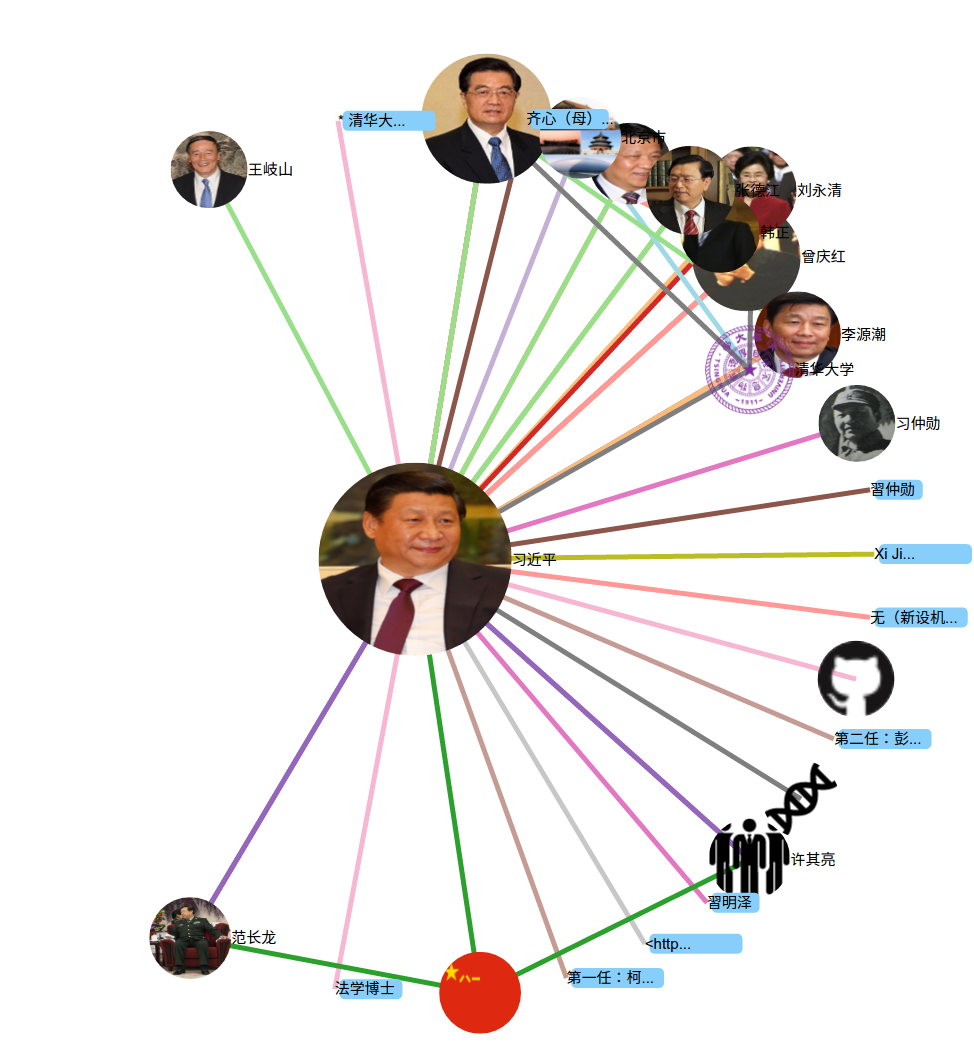
\includegraphics[width=0.5\hsize]{pic/pkubase.png}
}

\frame{
  \begin{columns}[c]
   \column{.3\hsize}
   \column{.4\hsize}
   \begin{block}{}
    \centering \Large Thanks \\ 
    \vspace{0.5em}
    \centering \Large Q \& A \\ 
   \end{block}
   \column{.3\hsize}
  \end{columns}
}

\frame{
  \frametitle{Append}
}

\end{document}